\chapter{Le prototype de calorimètre à lecture semi-digitale}
Dans ce charpitre le prototype de calorimètre à lecture semi-digitale qui a été construit au sein de l'instituts de physiques nucléaire de Lyon en 2011 sera décrit. Ce prototype a été testé lors de plusieurs campagnes de test en faisceau au CERN. Pendant ces tests, le prototype a été éxposé à un flux de particules tel que des pions, des protons, des muons et des électrons. Nous détaillerons les différents méthodes utilisées pour reconstruire l'energie des hadrons incidents. 
\minitoc
\newpage

%%%%%%%%%%%%%%%%%%%%%%%%%%%%%%%%%%%%%%%%%%%%%%%

\section{Les gerbes hadroniques}

\begin{figure}[!h]
  \begin{center}
    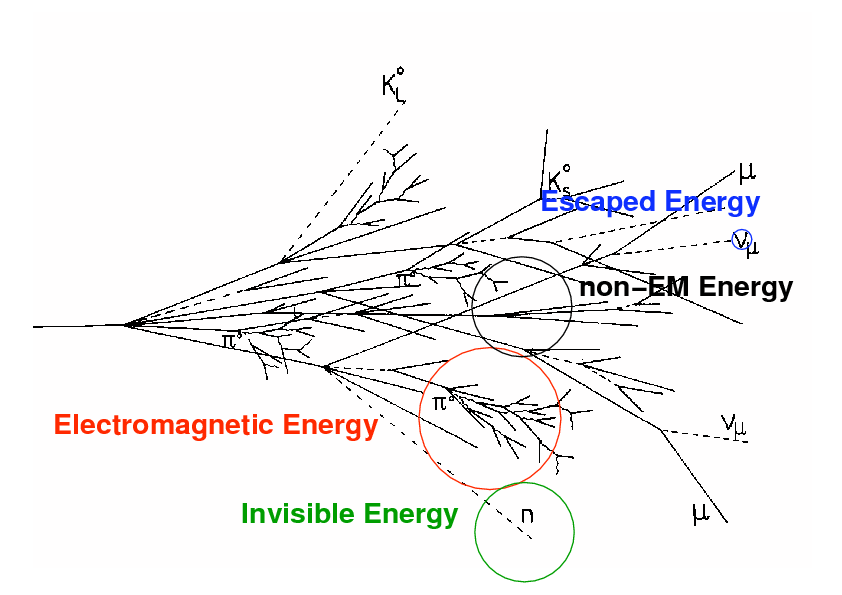
\includegraphics[width=.8\textwidth]{SDHCAL/figs/had-shower.png}
    \caption{Schéma du développement d'une gerbe hadronic.}
    \label{fig:showerScheme}
  \end{center}
\end{figure}

%%%%%%%%%%%%%%%%%%%%%%%%%%%%%%%%%%%%%%%%%%%%%%%

\section{Le SDHCAL}

\begin{figure}[!h]
  \begin{center}
    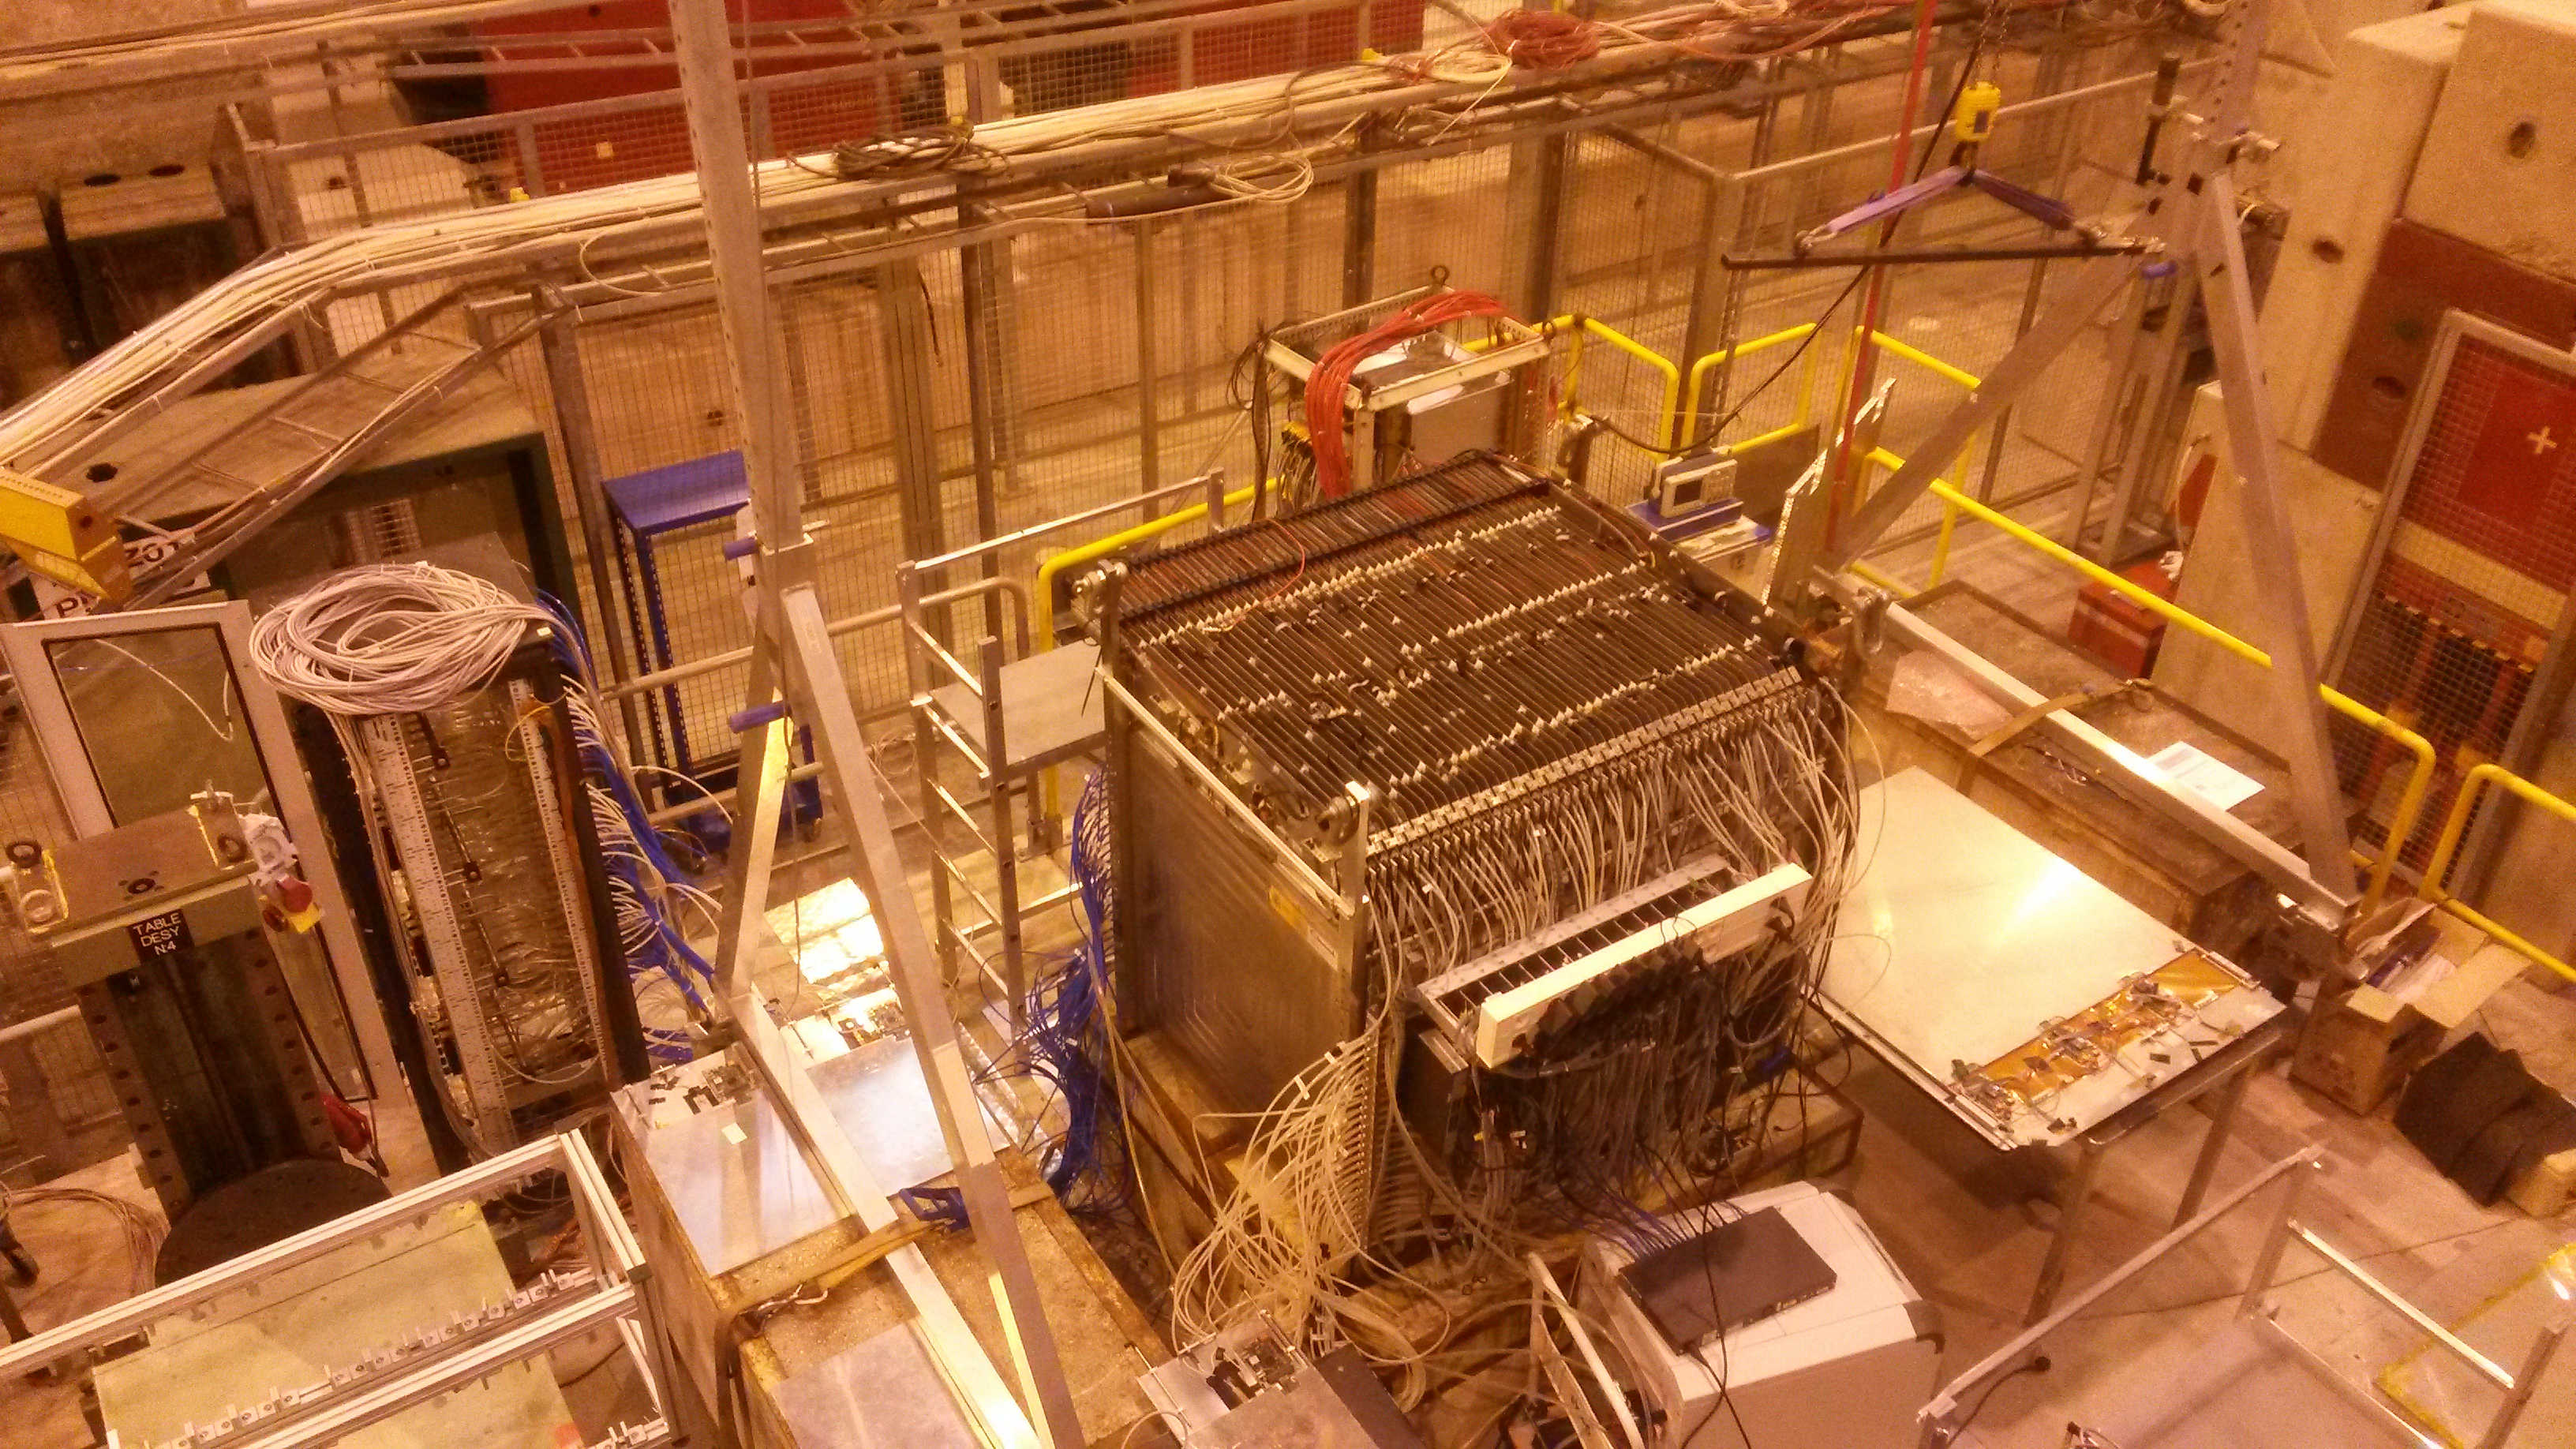
\includegraphics[width=.8\textwidth]{SDHCAL/figs/proto.jpg}
    \caption{Le prototype du calorimètre à lecture semi-digitale sur la ligne de faiceau H6 du CERN.}
    \label{fig:proto}
  \end{center}
\end{figure}

%%%%%%%%%%%%%%%%%%%%%%%%%%%%%%%%%%%%%%%%%%%%%%%

\section{Les chambres à plaques de verre résistif}

\begin{figure}[!h]
  \begin{center}
    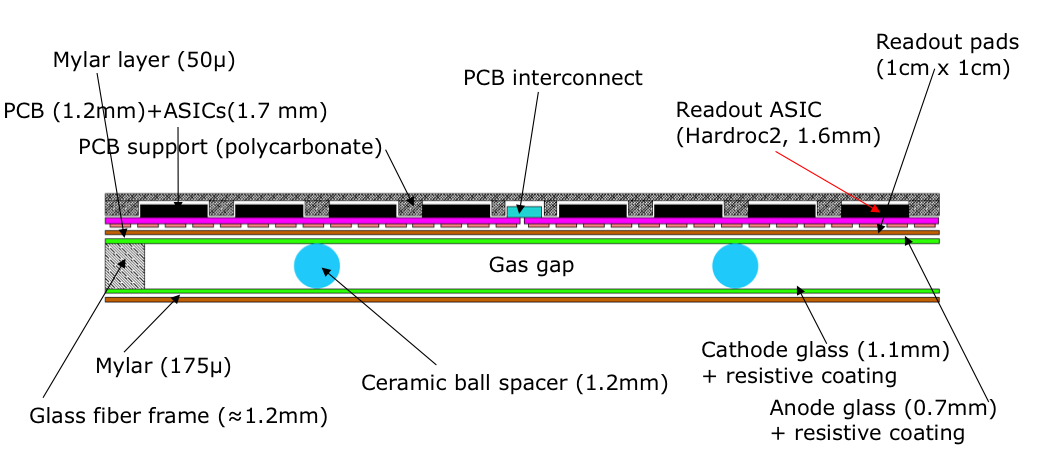
\includegraphics[width=.8\textwidth]{SDHCAL/figs/GRPC-K7.png}
    \caption{Schéma d'une GRPC.}
    \label{fig:grpc}
  \end{center}
\end{figure}

\begin{figure}[!h]
  \begin{center}
    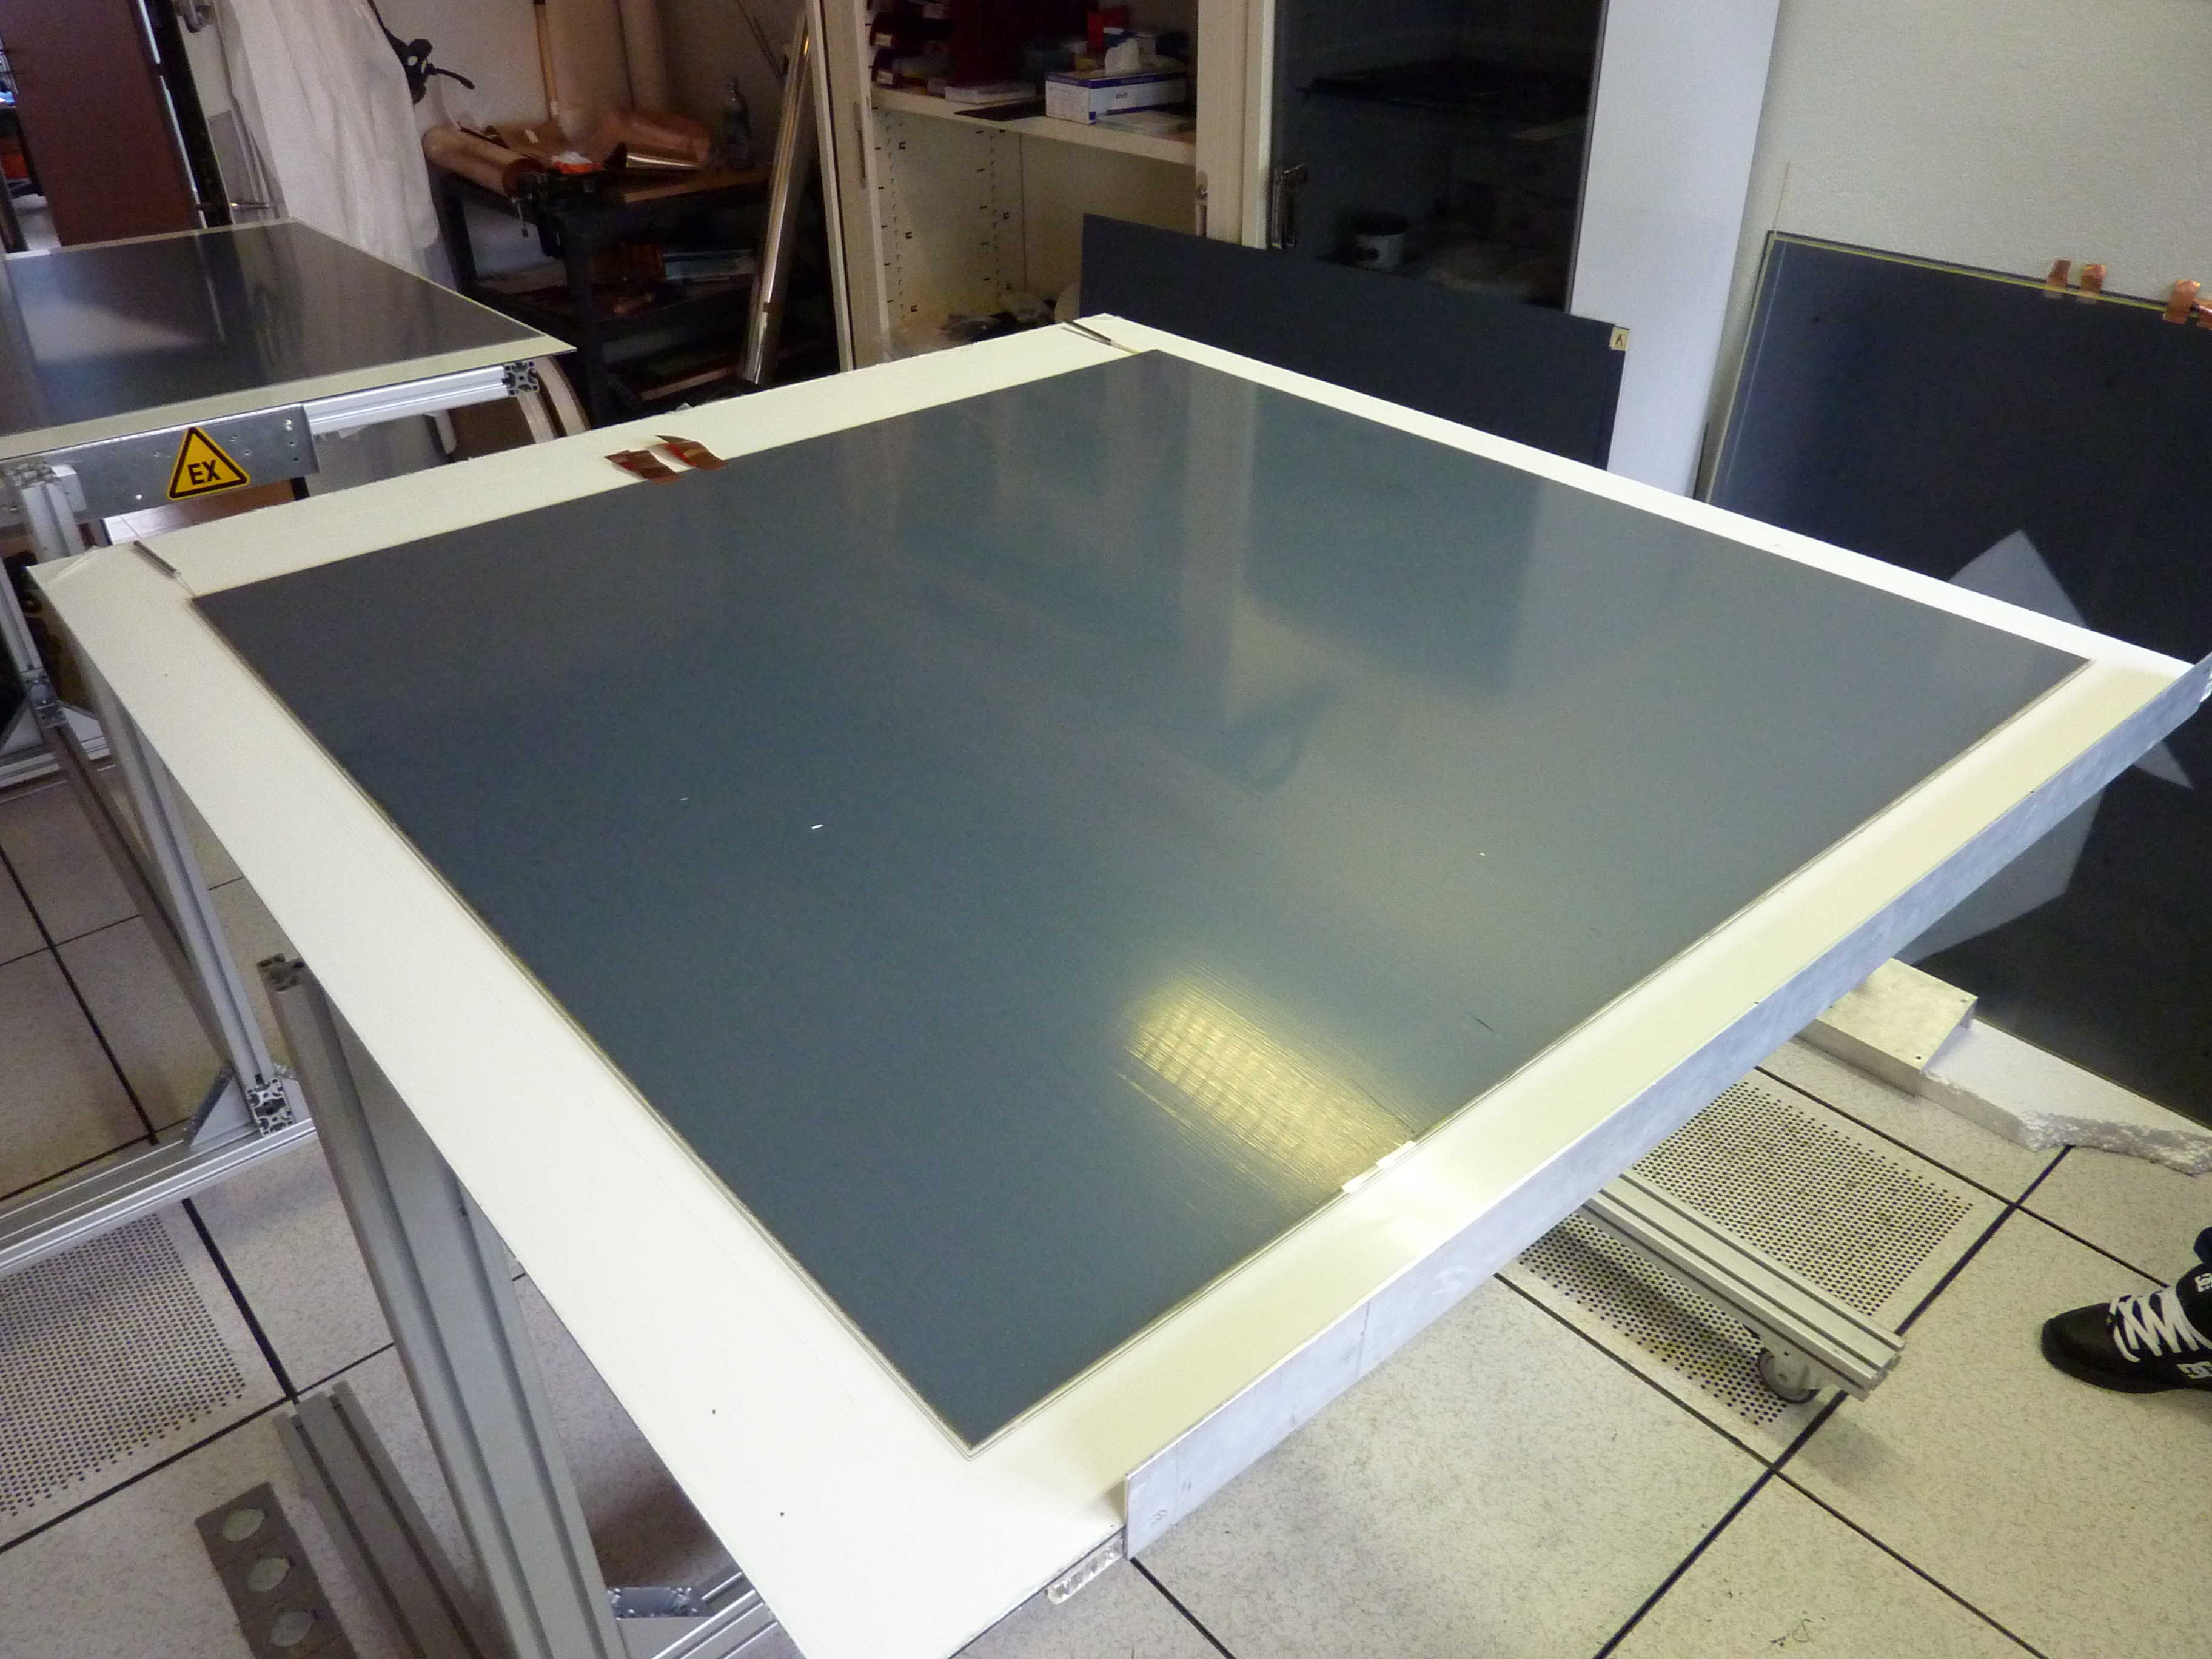
\includegraphics[width=.47\textwidth]{SDHCAL/figs/aLayer.jpg}
    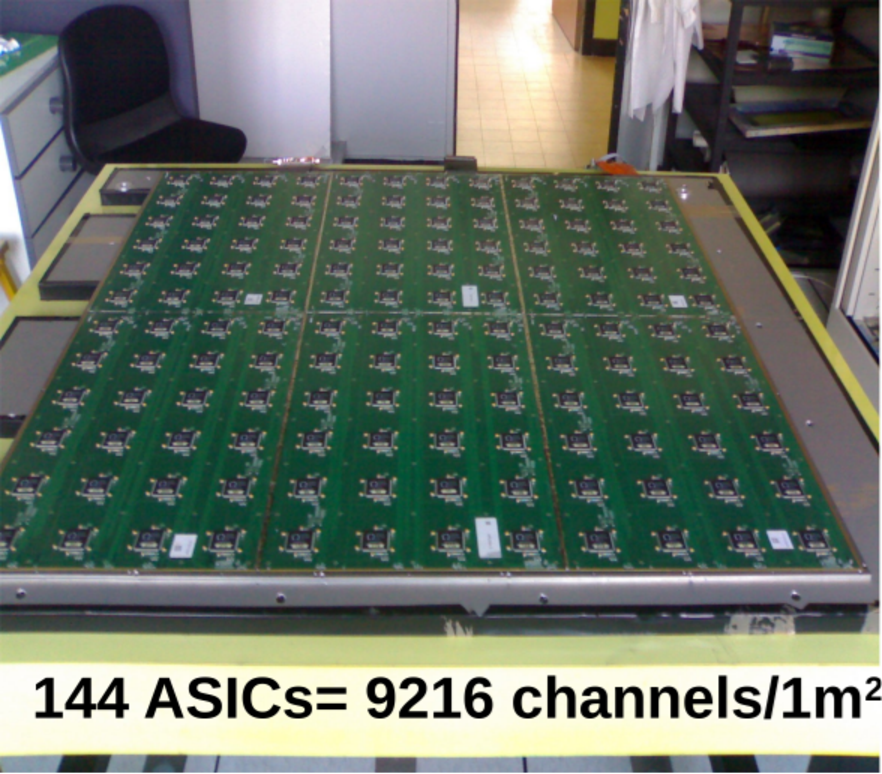
\includegraphics[width=.4\textwidth]{SDHCAL/figs/layer_electronic2.pdf}
    \caption{Photo de plan de rpc et d'un plan d'électronique.}
    \label{fig:layer}
  \end{center}
\end{figure}

%%%%%%%%%%%%%%%%%%%%%%%%%%%%%%%%%%%%%%%%%%%%%%%

\section{Reconstruction de l'énergie dans le SDHCAL}

\subsection{Reconstruction des évenements}
\begin{figure}[!h]
  \begin{center}
    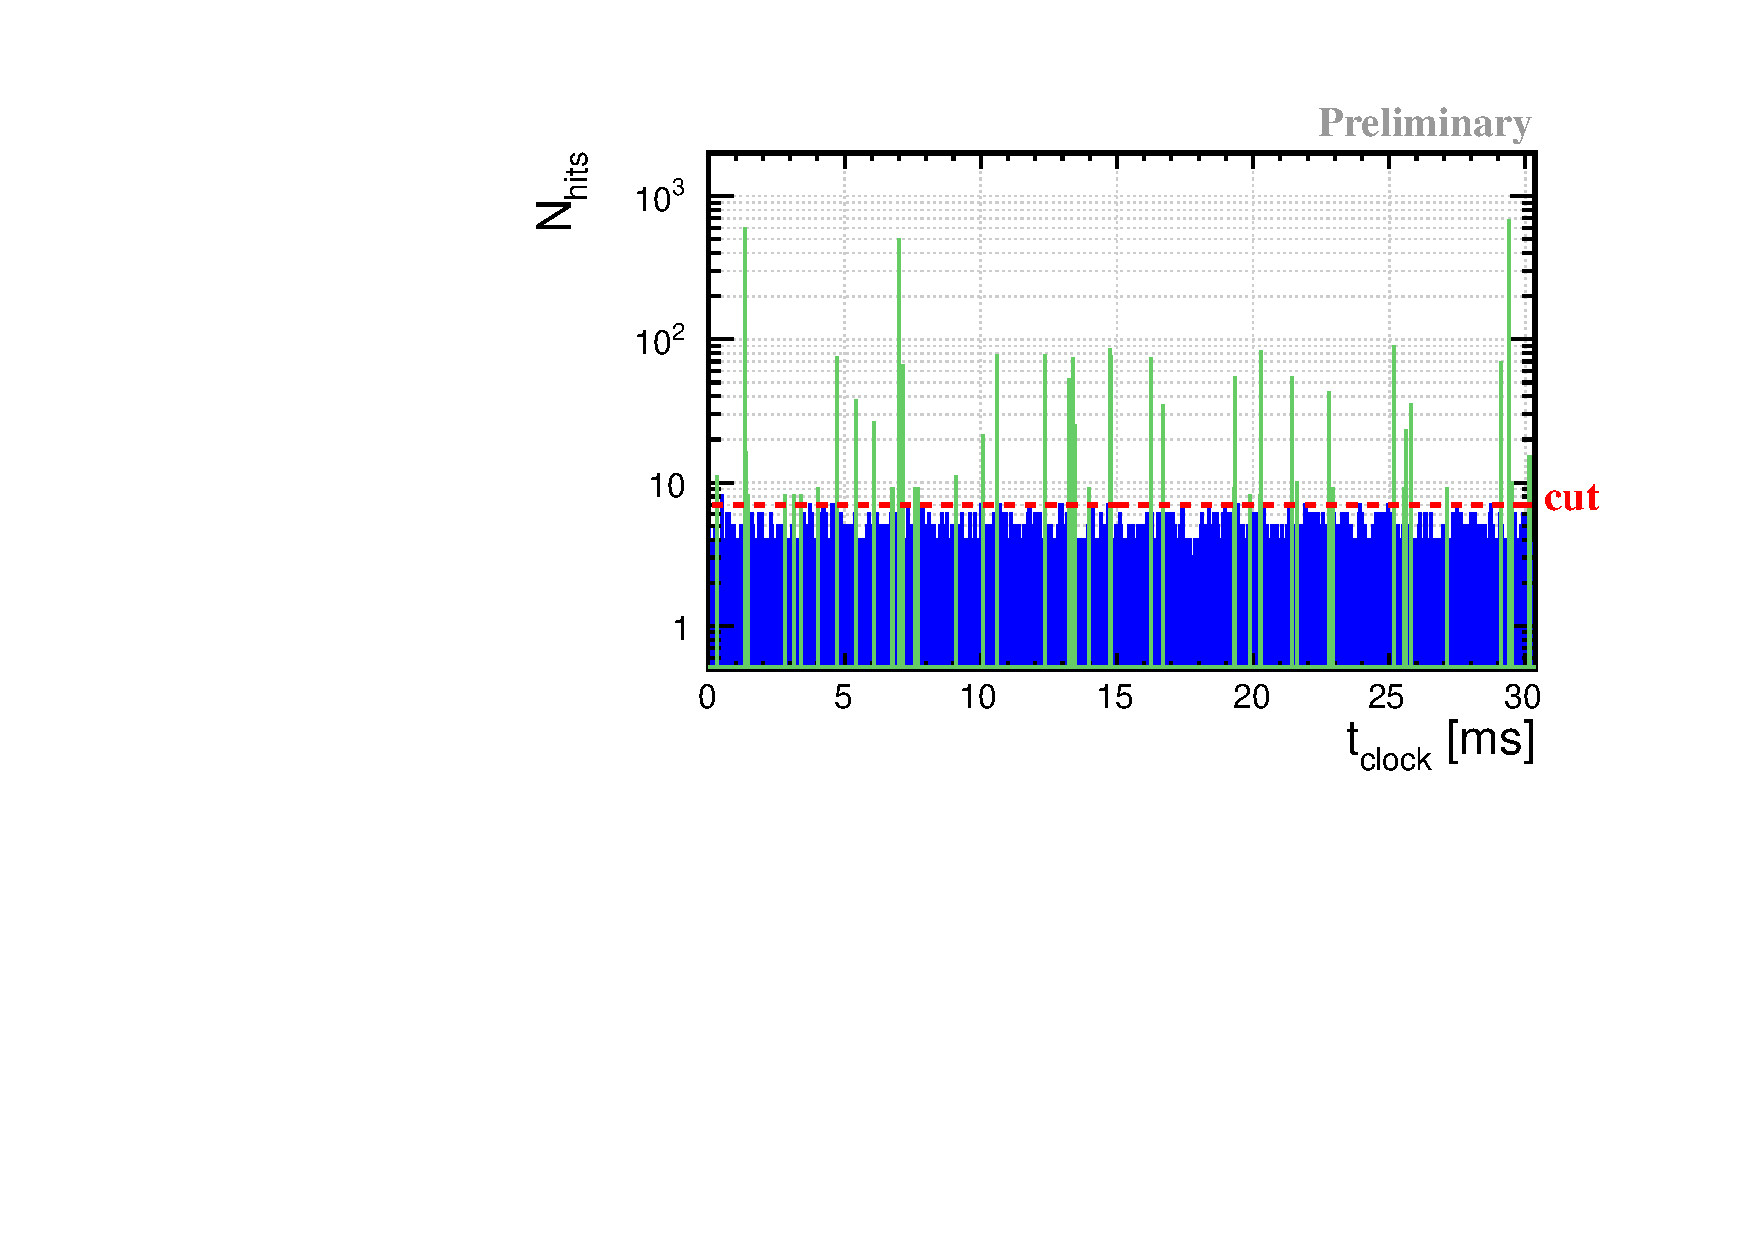
\includegraphics[width=.8\textwidth]{SDHCAL/figs/time_spectrum.pdf}
    \caption{Histogram des temps dans un trigger.}
    \label{fig:time_spectrum}
  \end{center}
\end{figure}

\subsection{Sélection des gerbes hadroniques}
\begin{figure}[!h]
  \begin{center}
    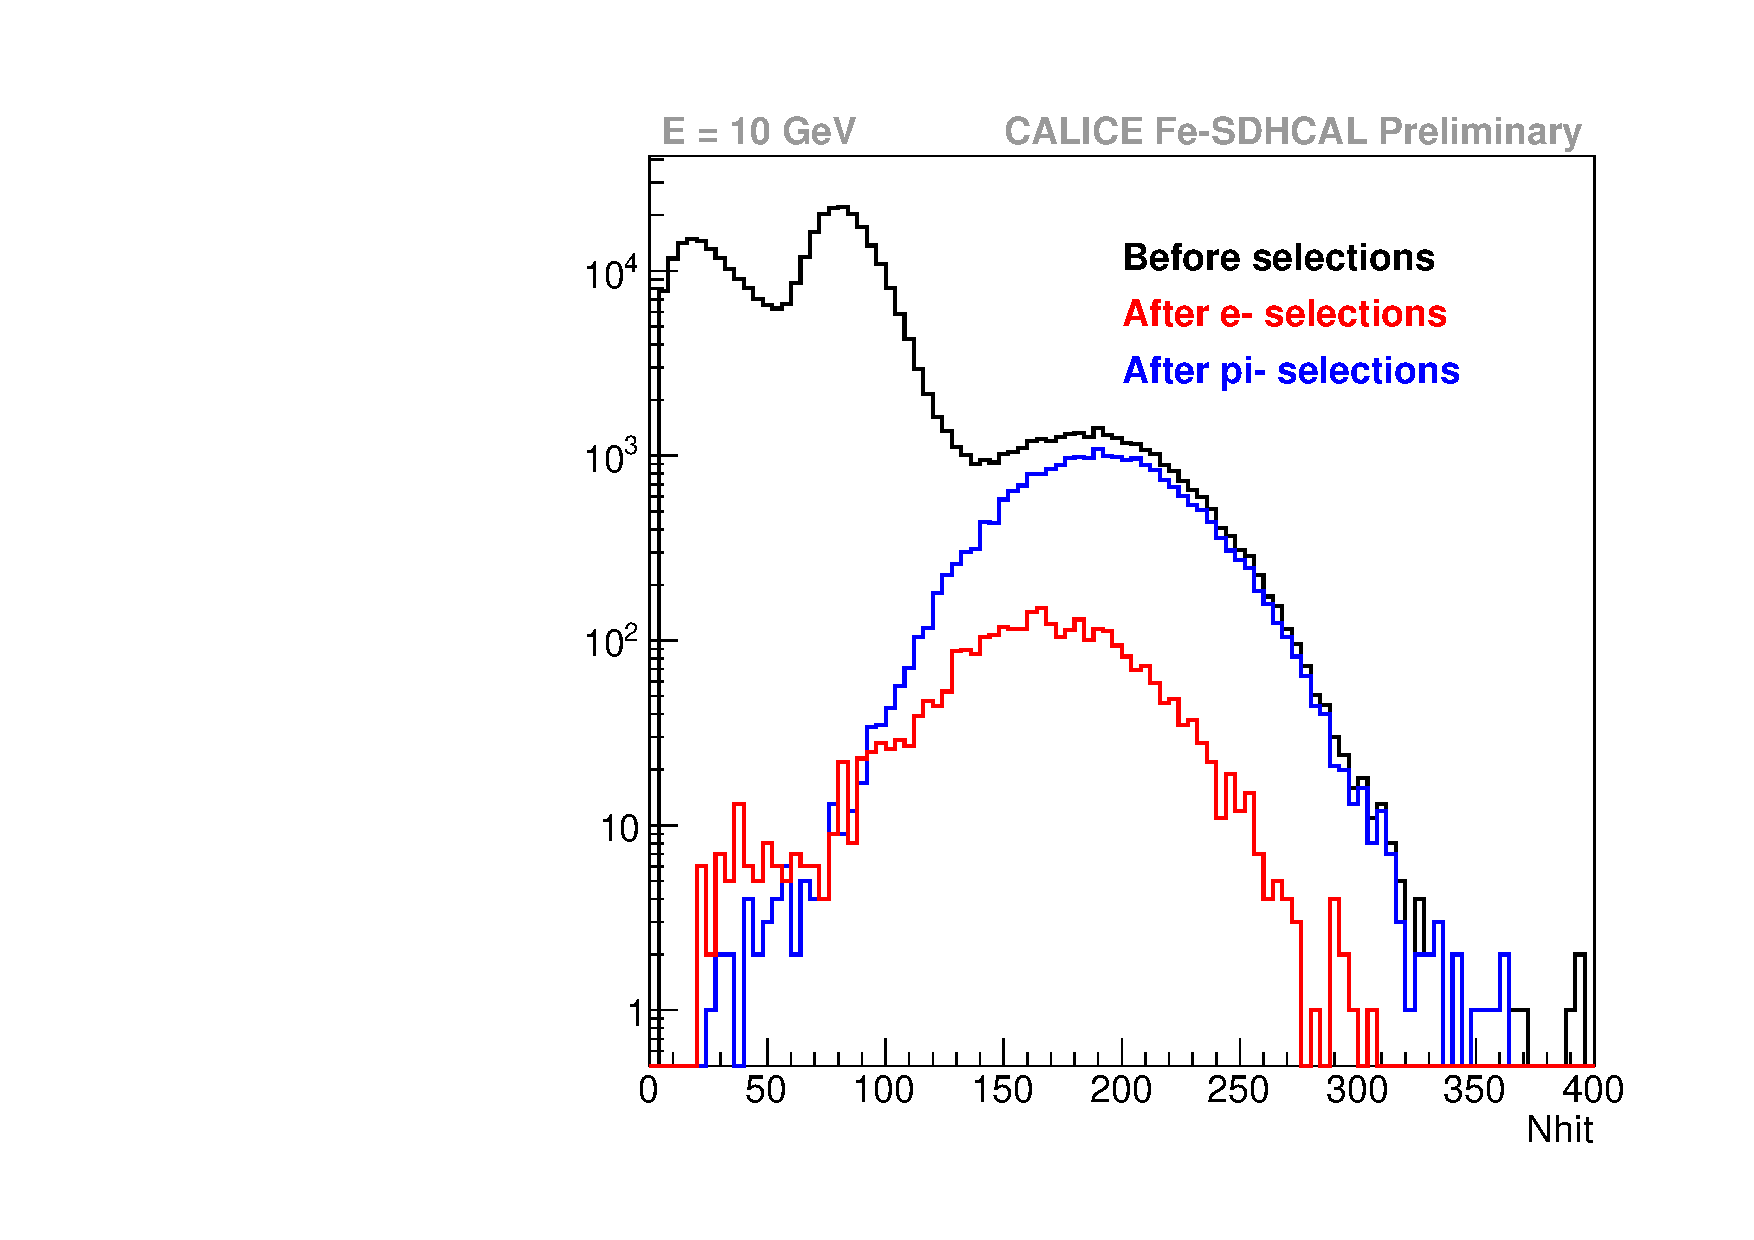
\includegraphics[width=.45\textwidth]{SDHCAL/figs/selection715693.pdf}
    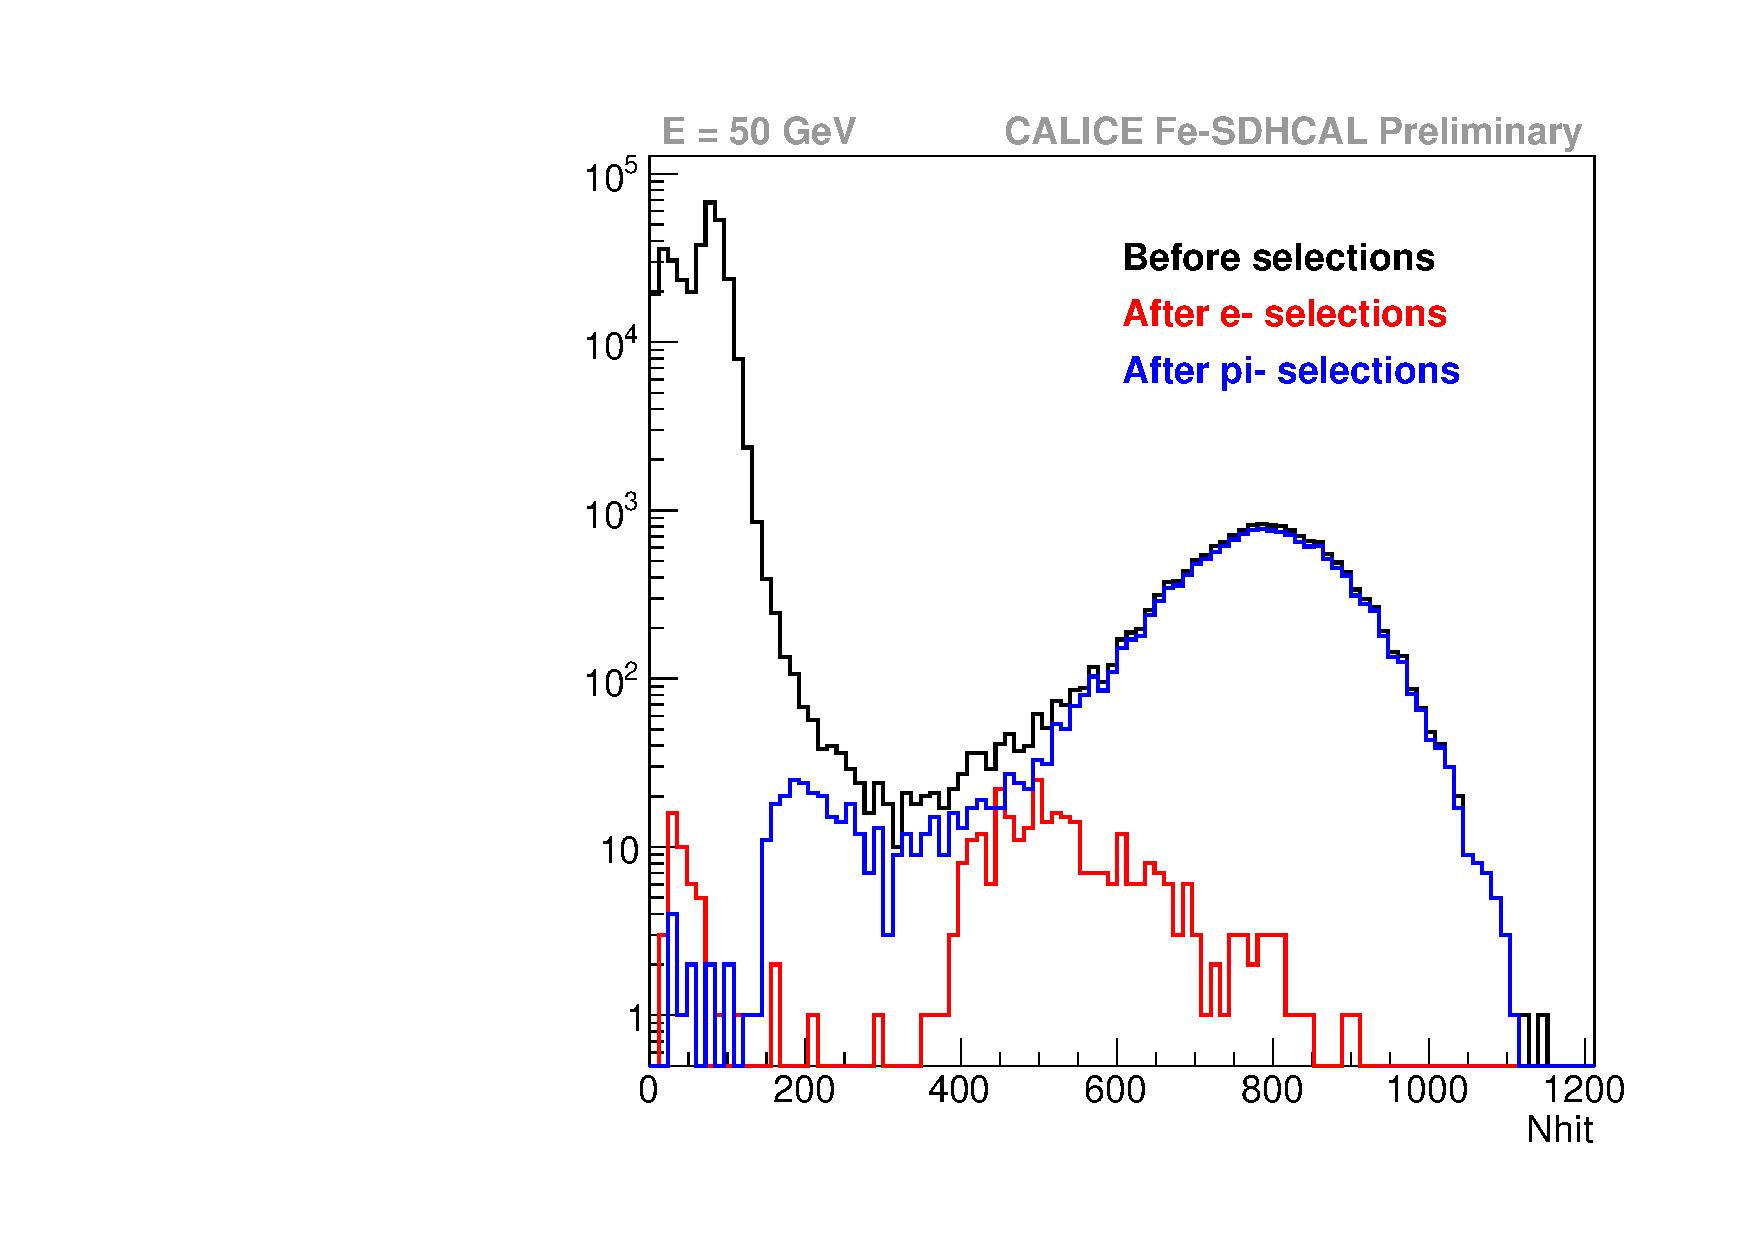
\includegraphics[width=.45\textwidth]{SDHCAL/figs/selection715751.pdf}
    \caption{Selections des pions.}
    \label{fig:pion_selection}
  \end{center}
\end{figure}

\subsection{Calibration en fonction du temps}
\begin{figure}[!h]
  \begin{center}
    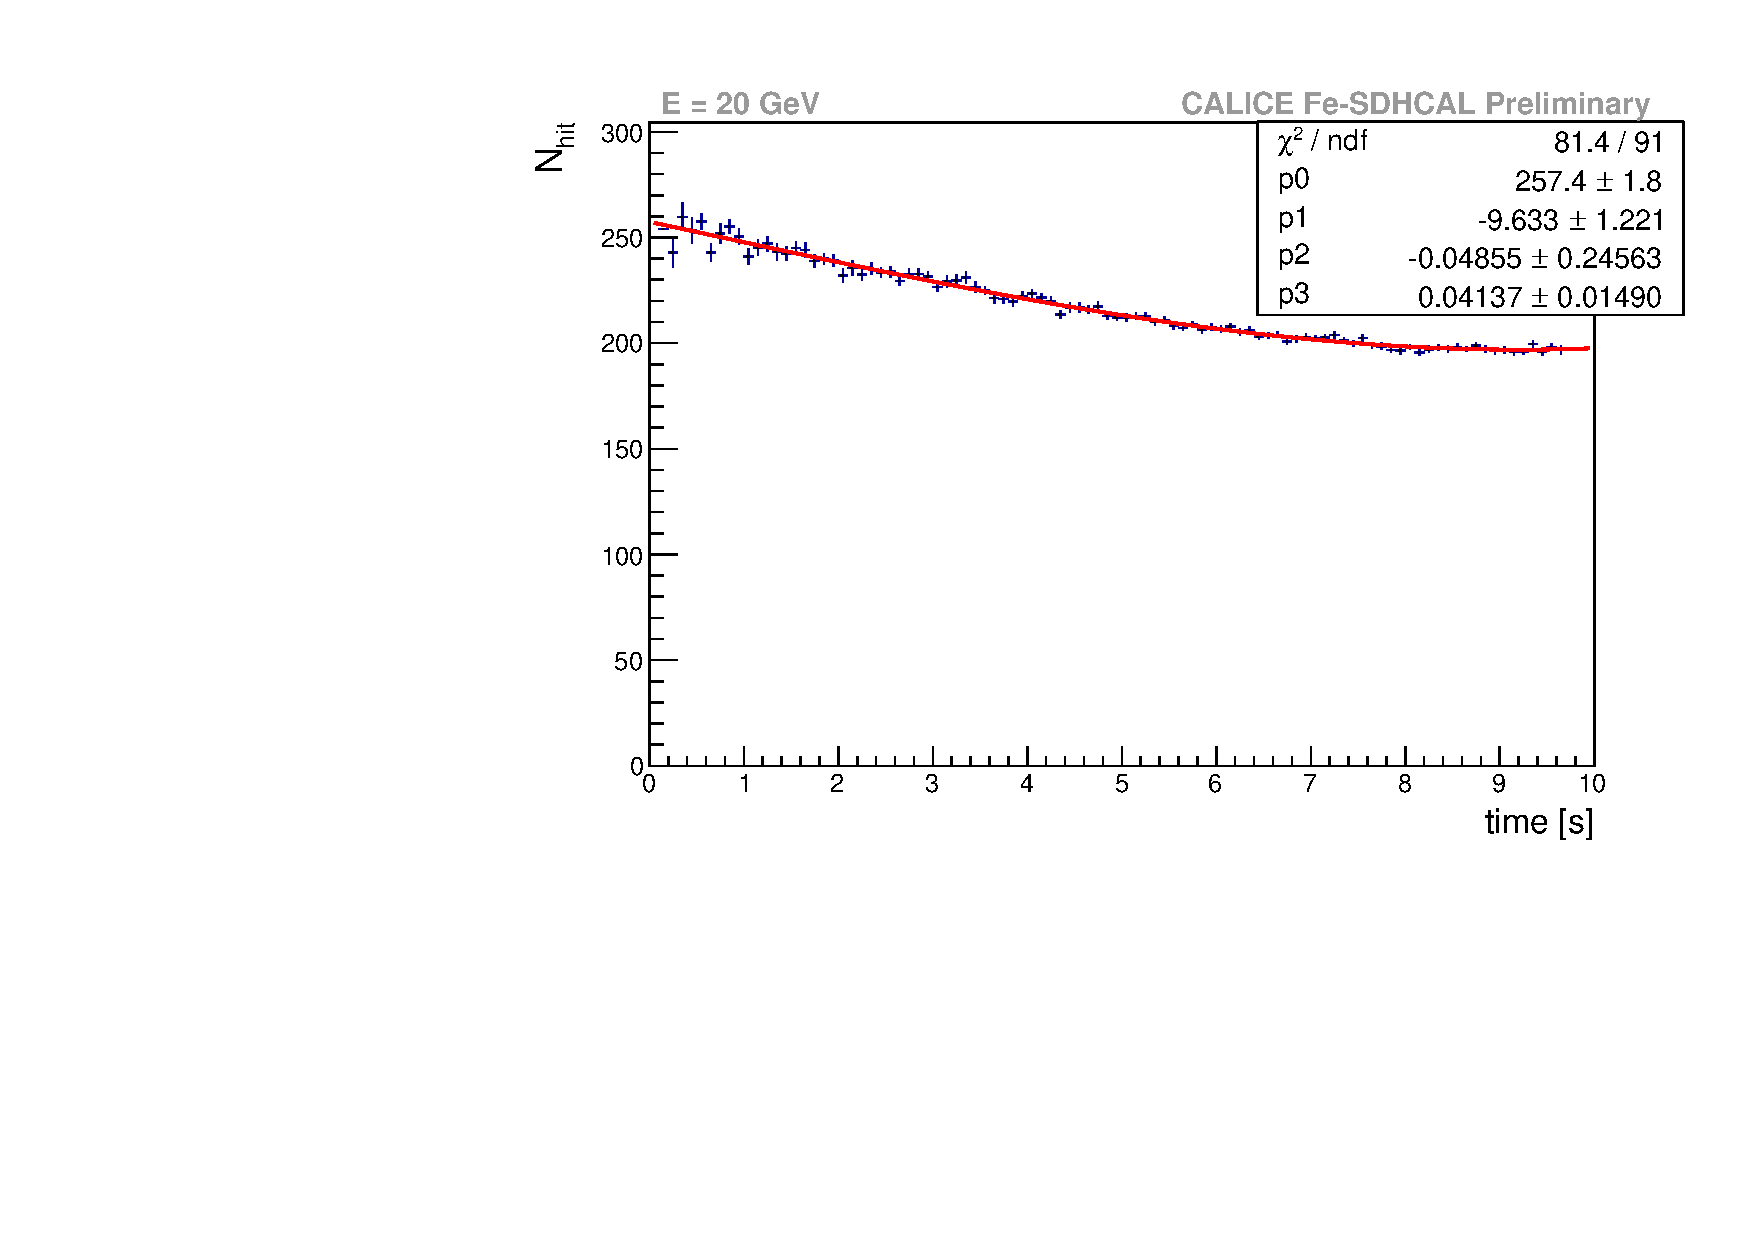
\includegraphics[width=.7\textwidth]{SDHCAL/figs/timeFit.pdf}
    \caption{Correction en focntion du temps.!! Figure avec électrons!!}
    \label{fig:time_correction}
  \end{center}
\end{figure}

\subsection{Reconstruction de l'énergie des pions}
\begin{figure}[!h]
  \begin{center}
    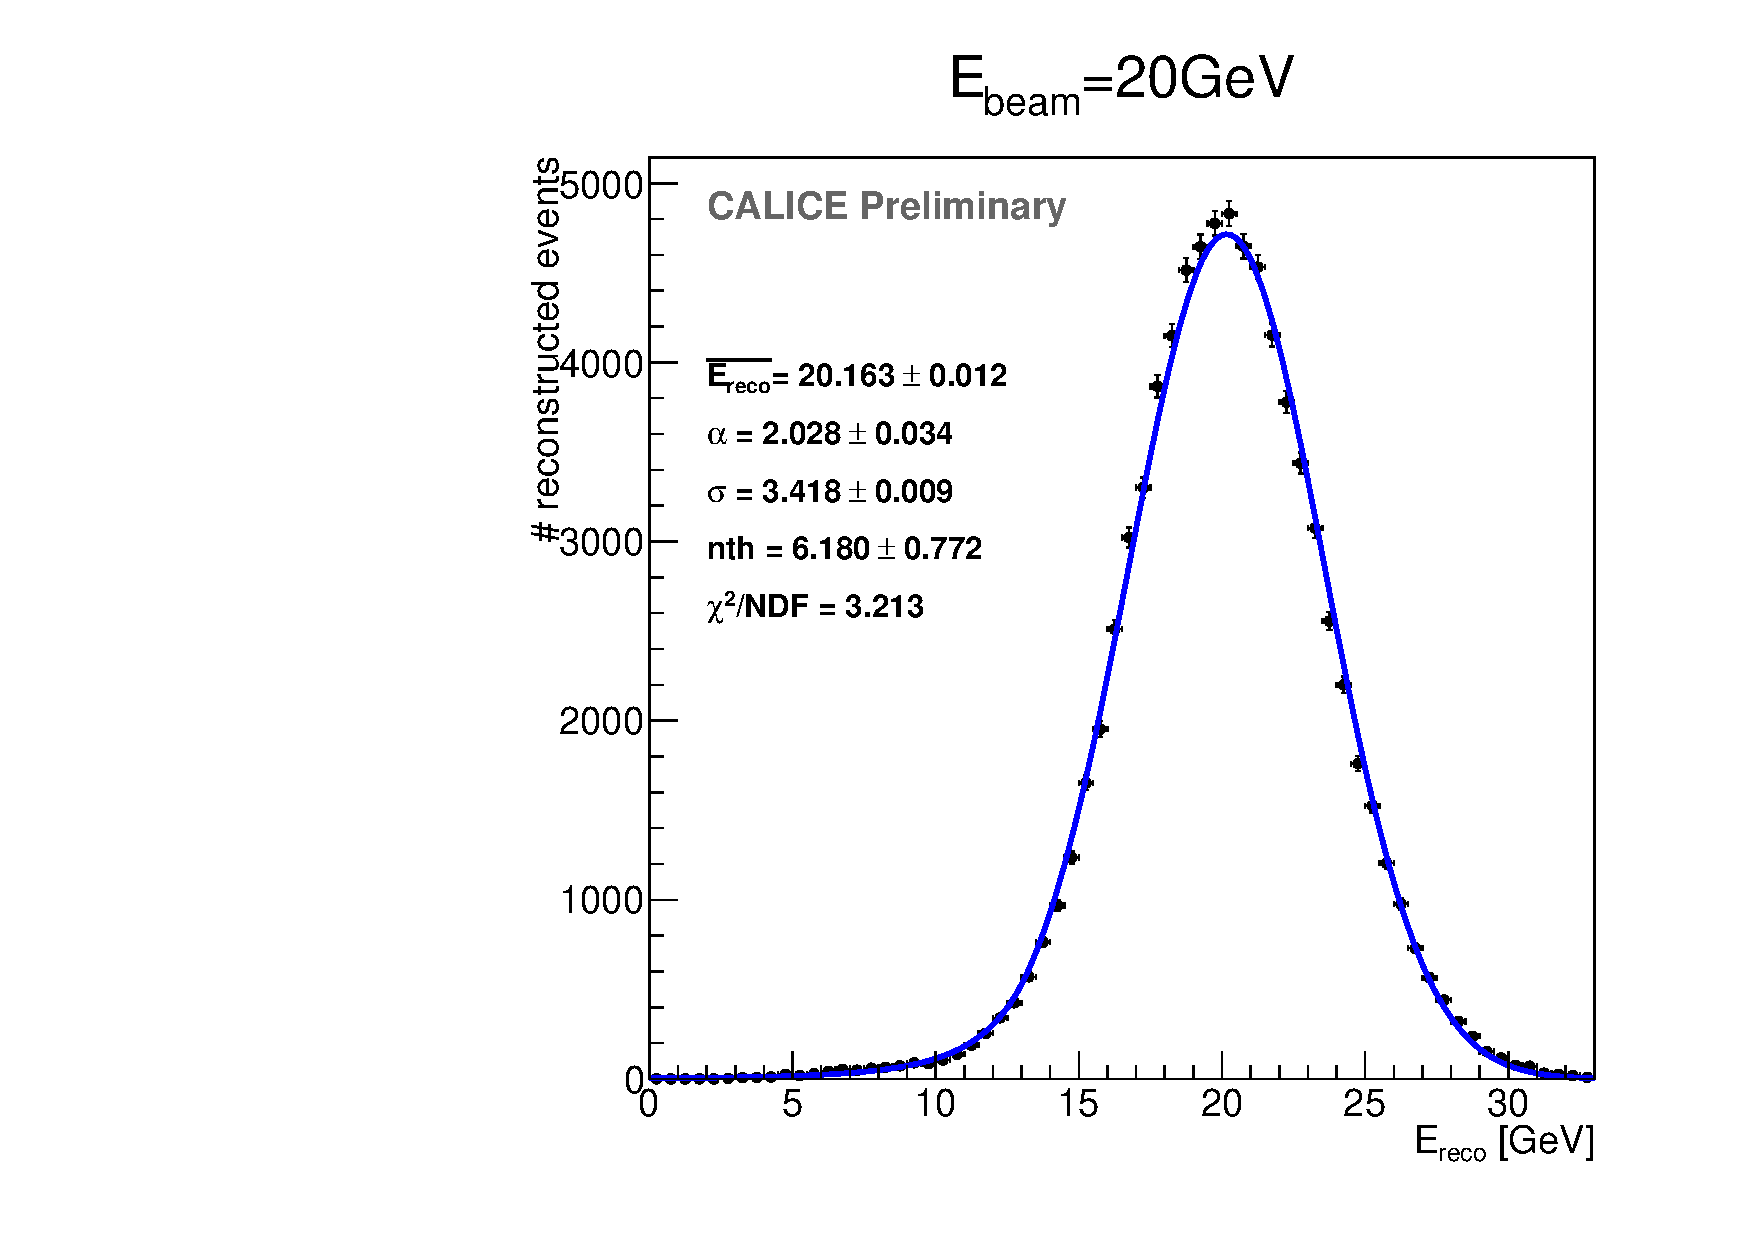
\includegraphics[width=.45\textwidth]{SDHCAL/figs/result20GeV.pdf}
    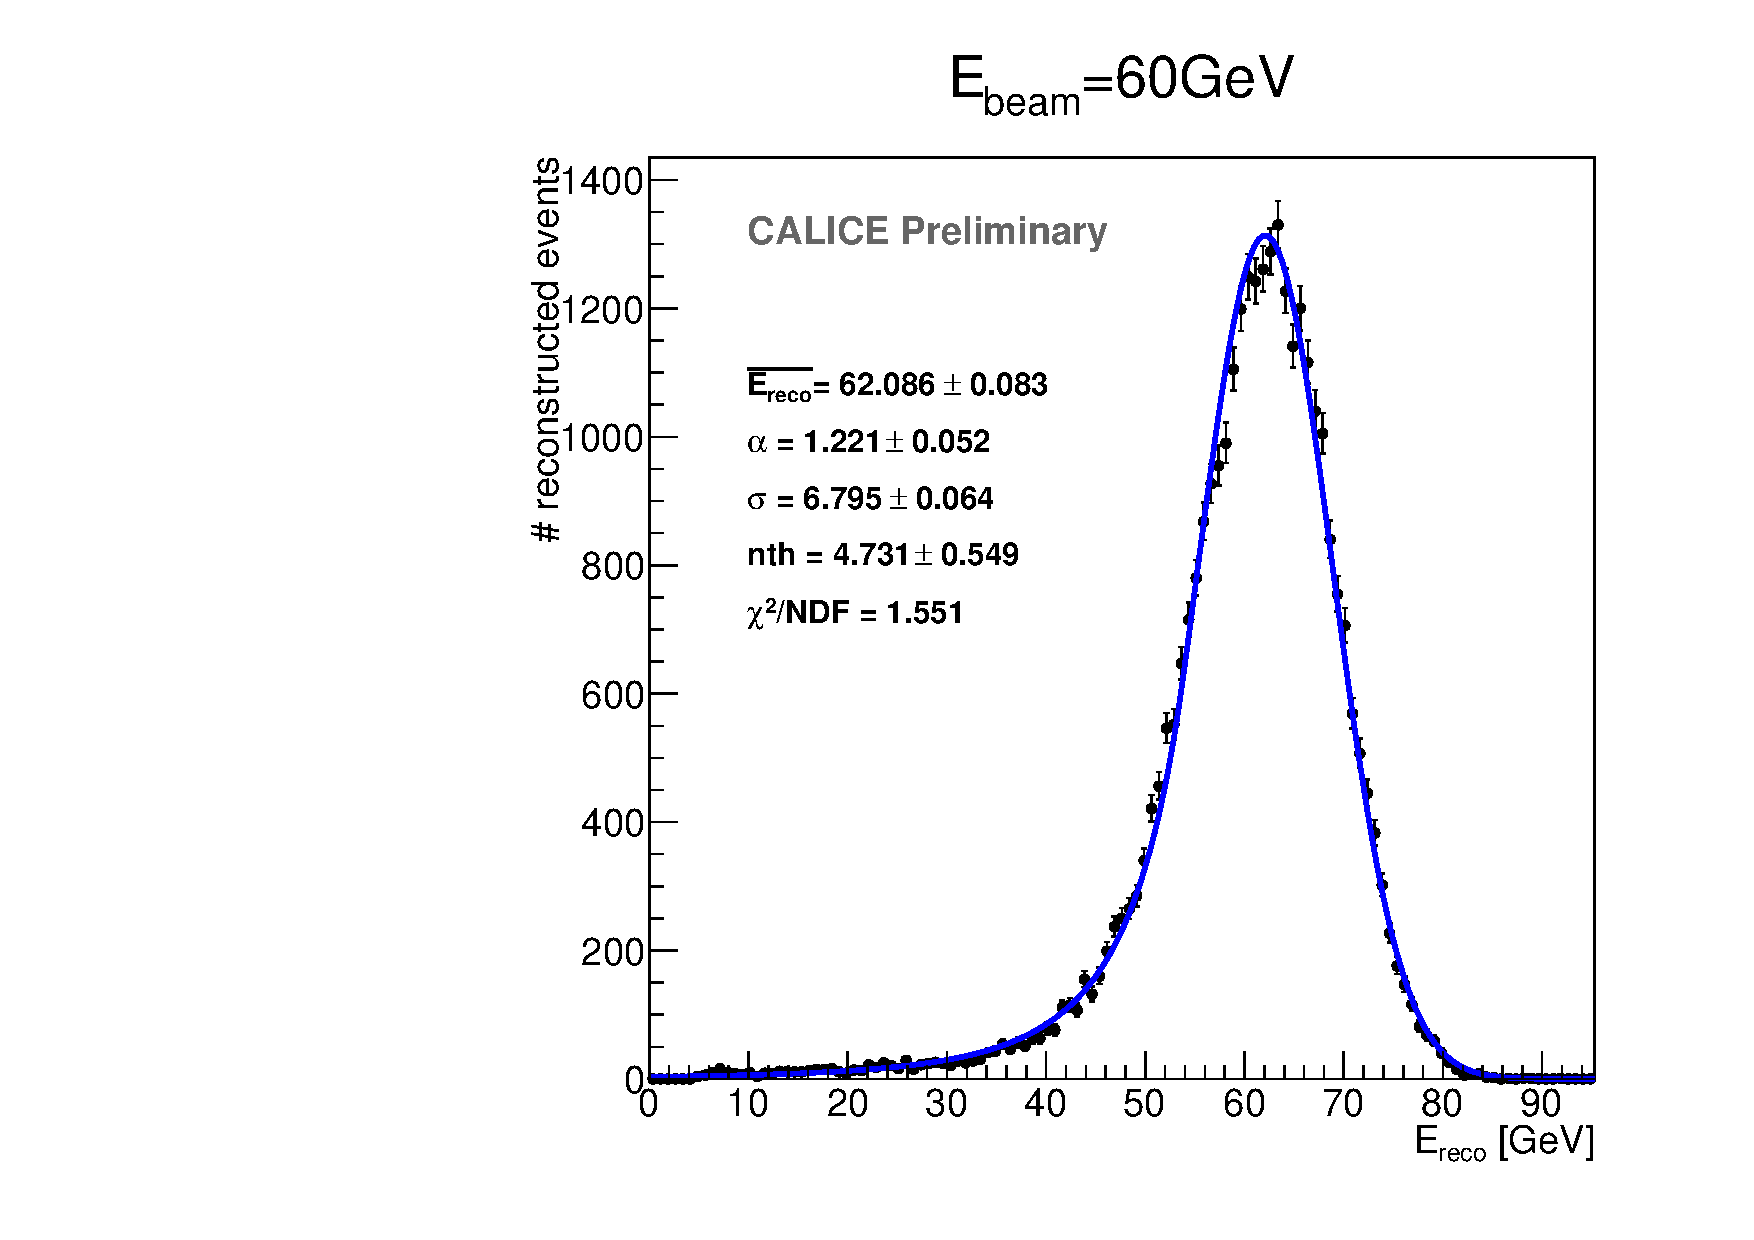
\includegraphics[width=.45\textwidth]{SDHCAL/figs/result60GeV.pdf}
    \caption{Distribution en energie.}
    \label{fig:energy_dist}
  \end{center}
\end{figure}

\begin{figure}[!h]
  \begin{center}
    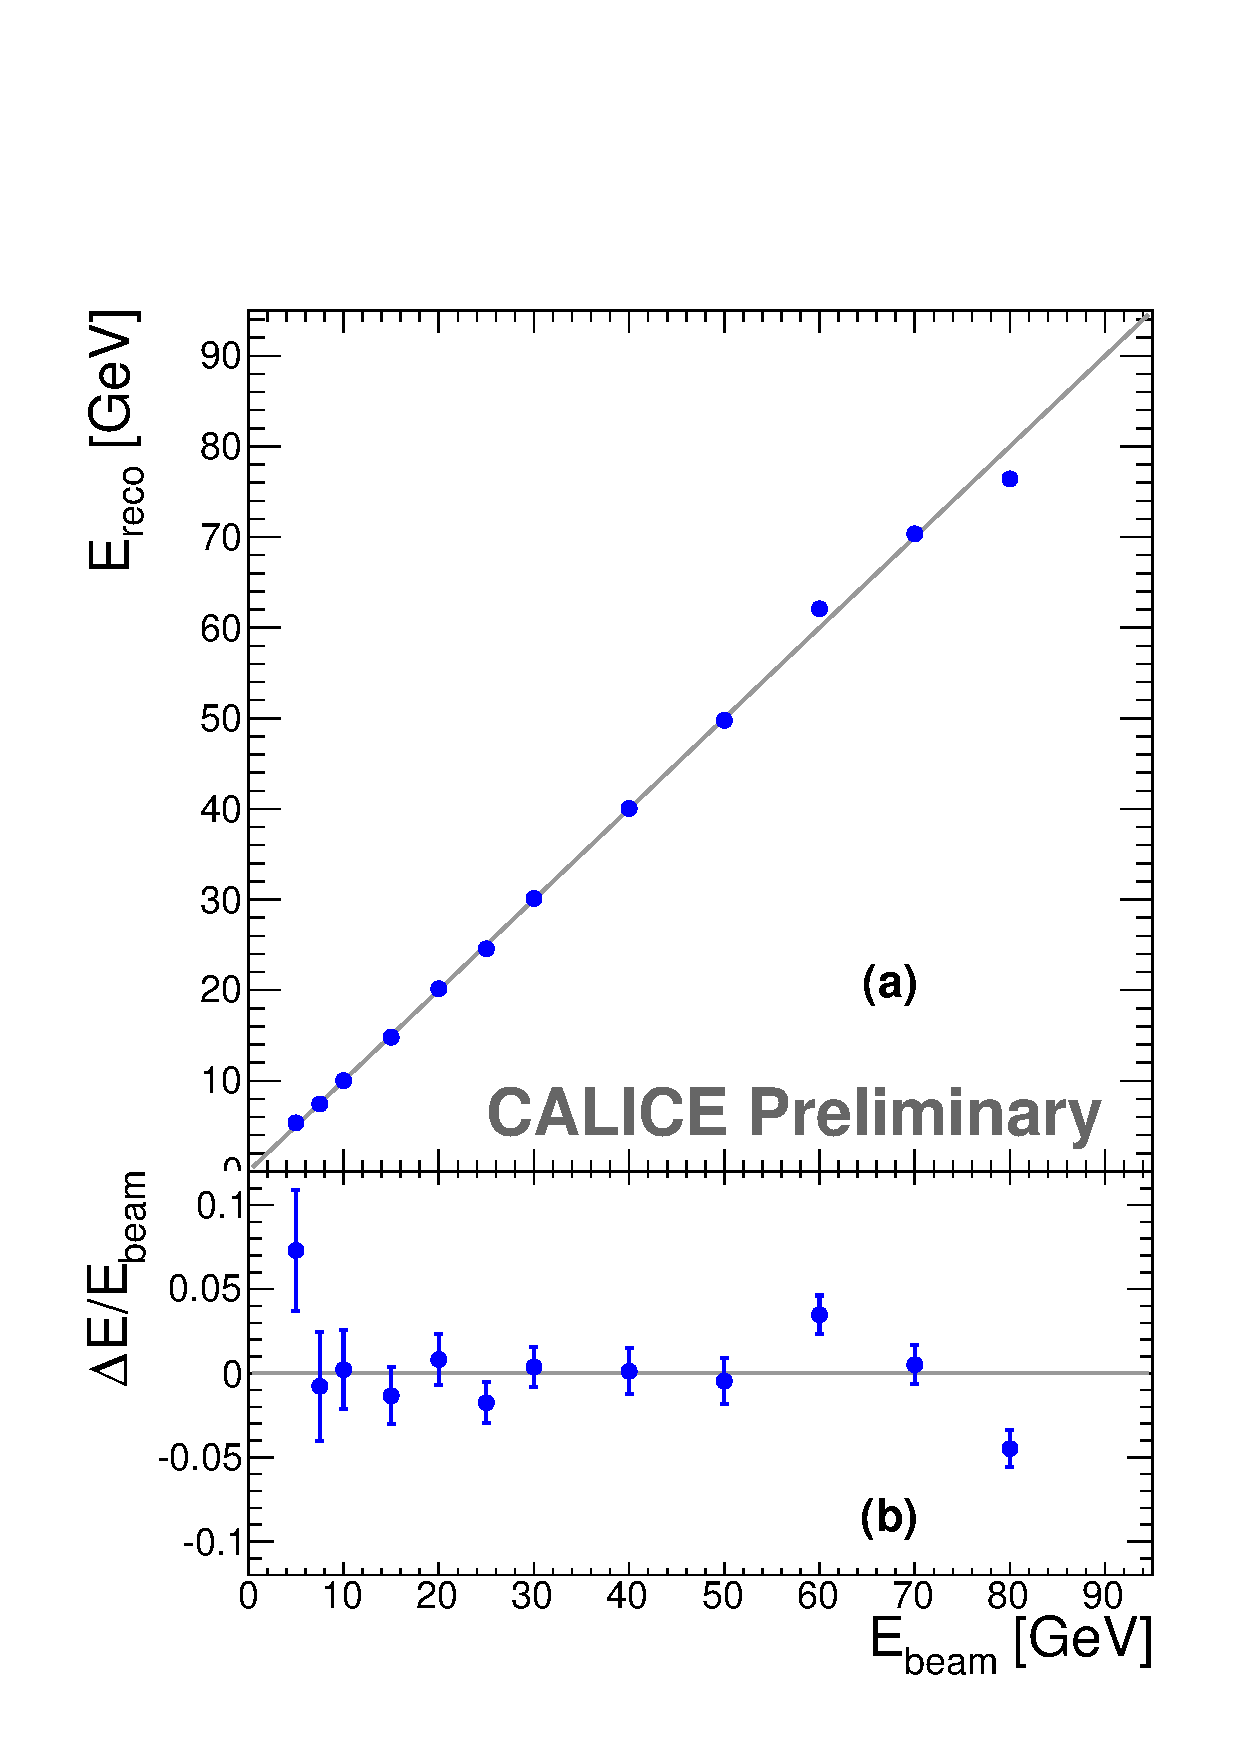
\includegraphics[width=.4\textwidth]{SDHCAL/figs/Energy-Linearity.pdf}
    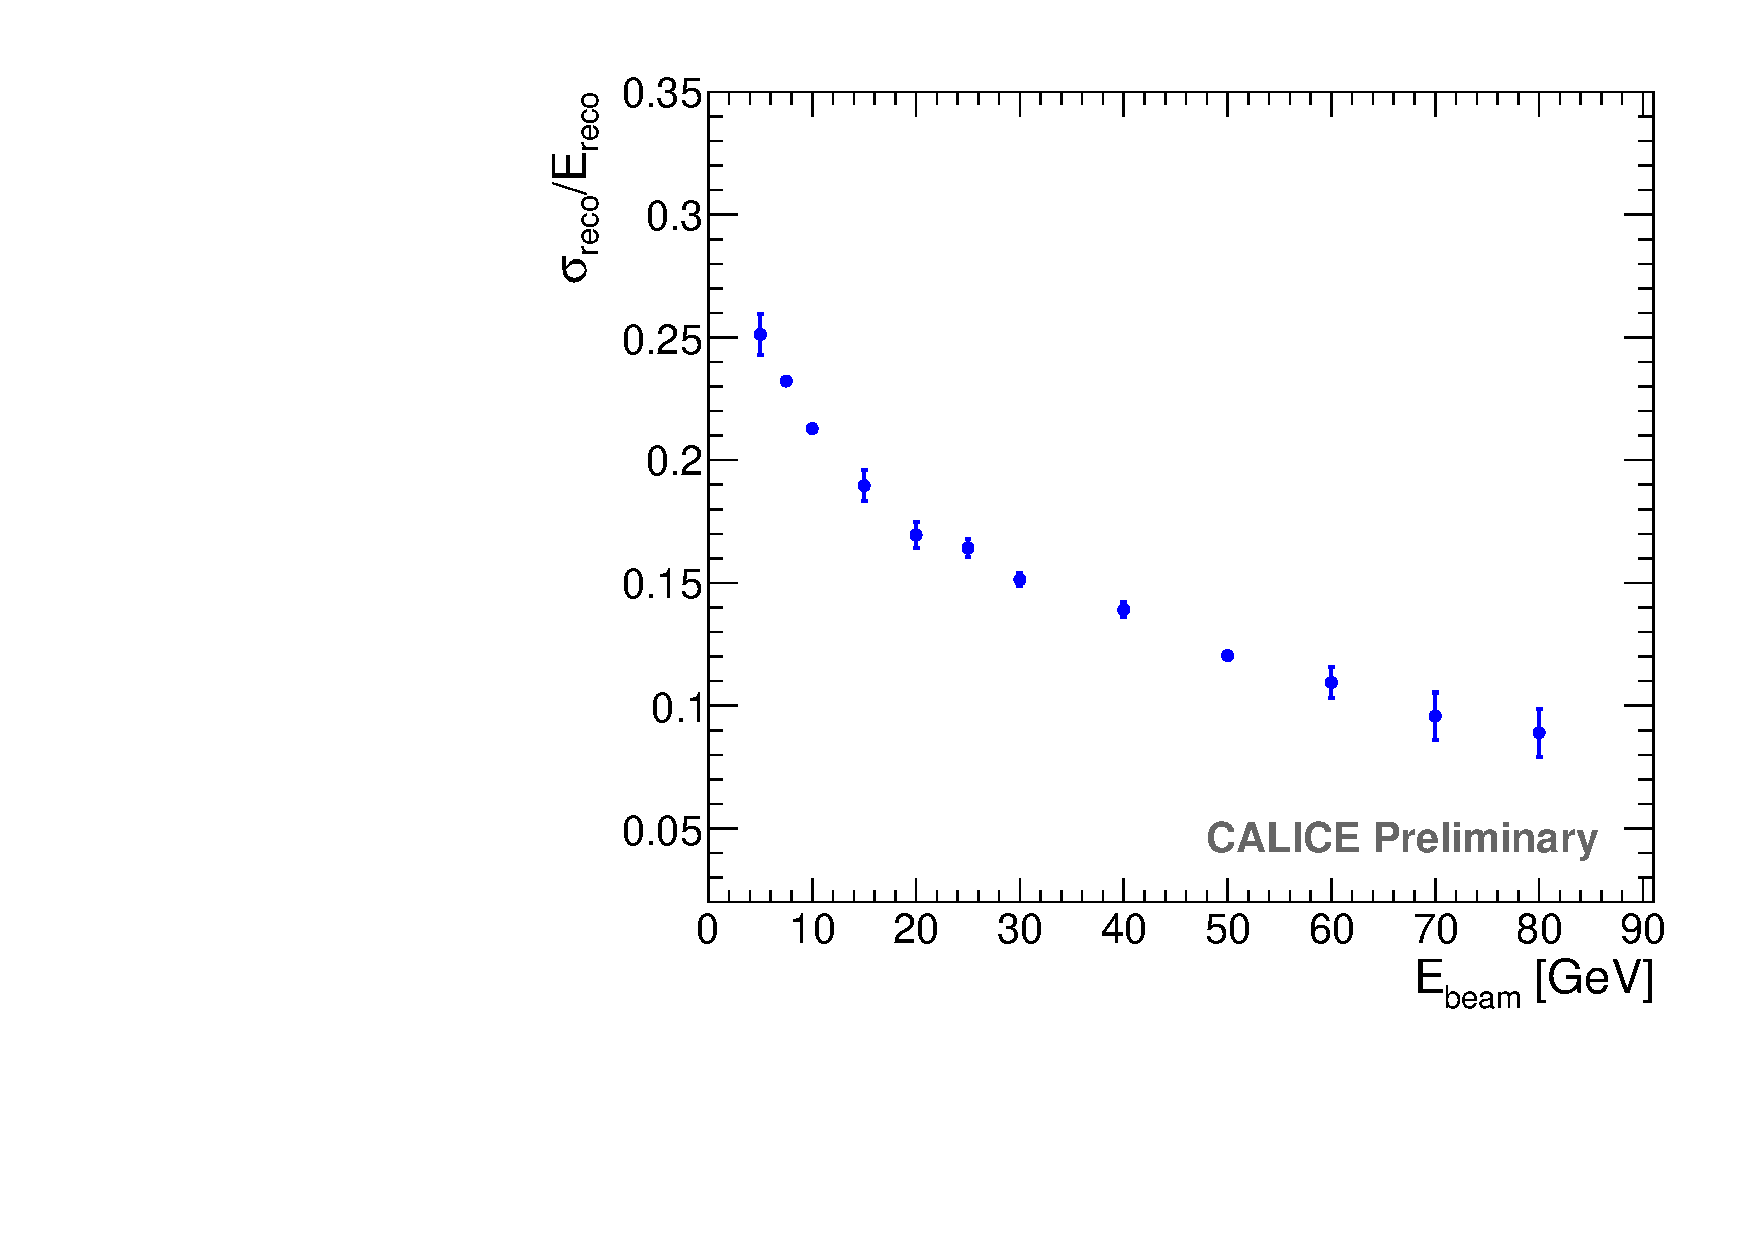
\includegraphics[width=.55\textwidth]{SDHCAL/figs/Energy-Resolution.pdf}
    \caption{Courbe de liéarité et résolution.}
    \label{fig:energy_lin-reso}
  \end{center}
\end{figure}

\begin{figure}[!h]
  \begin{center}
    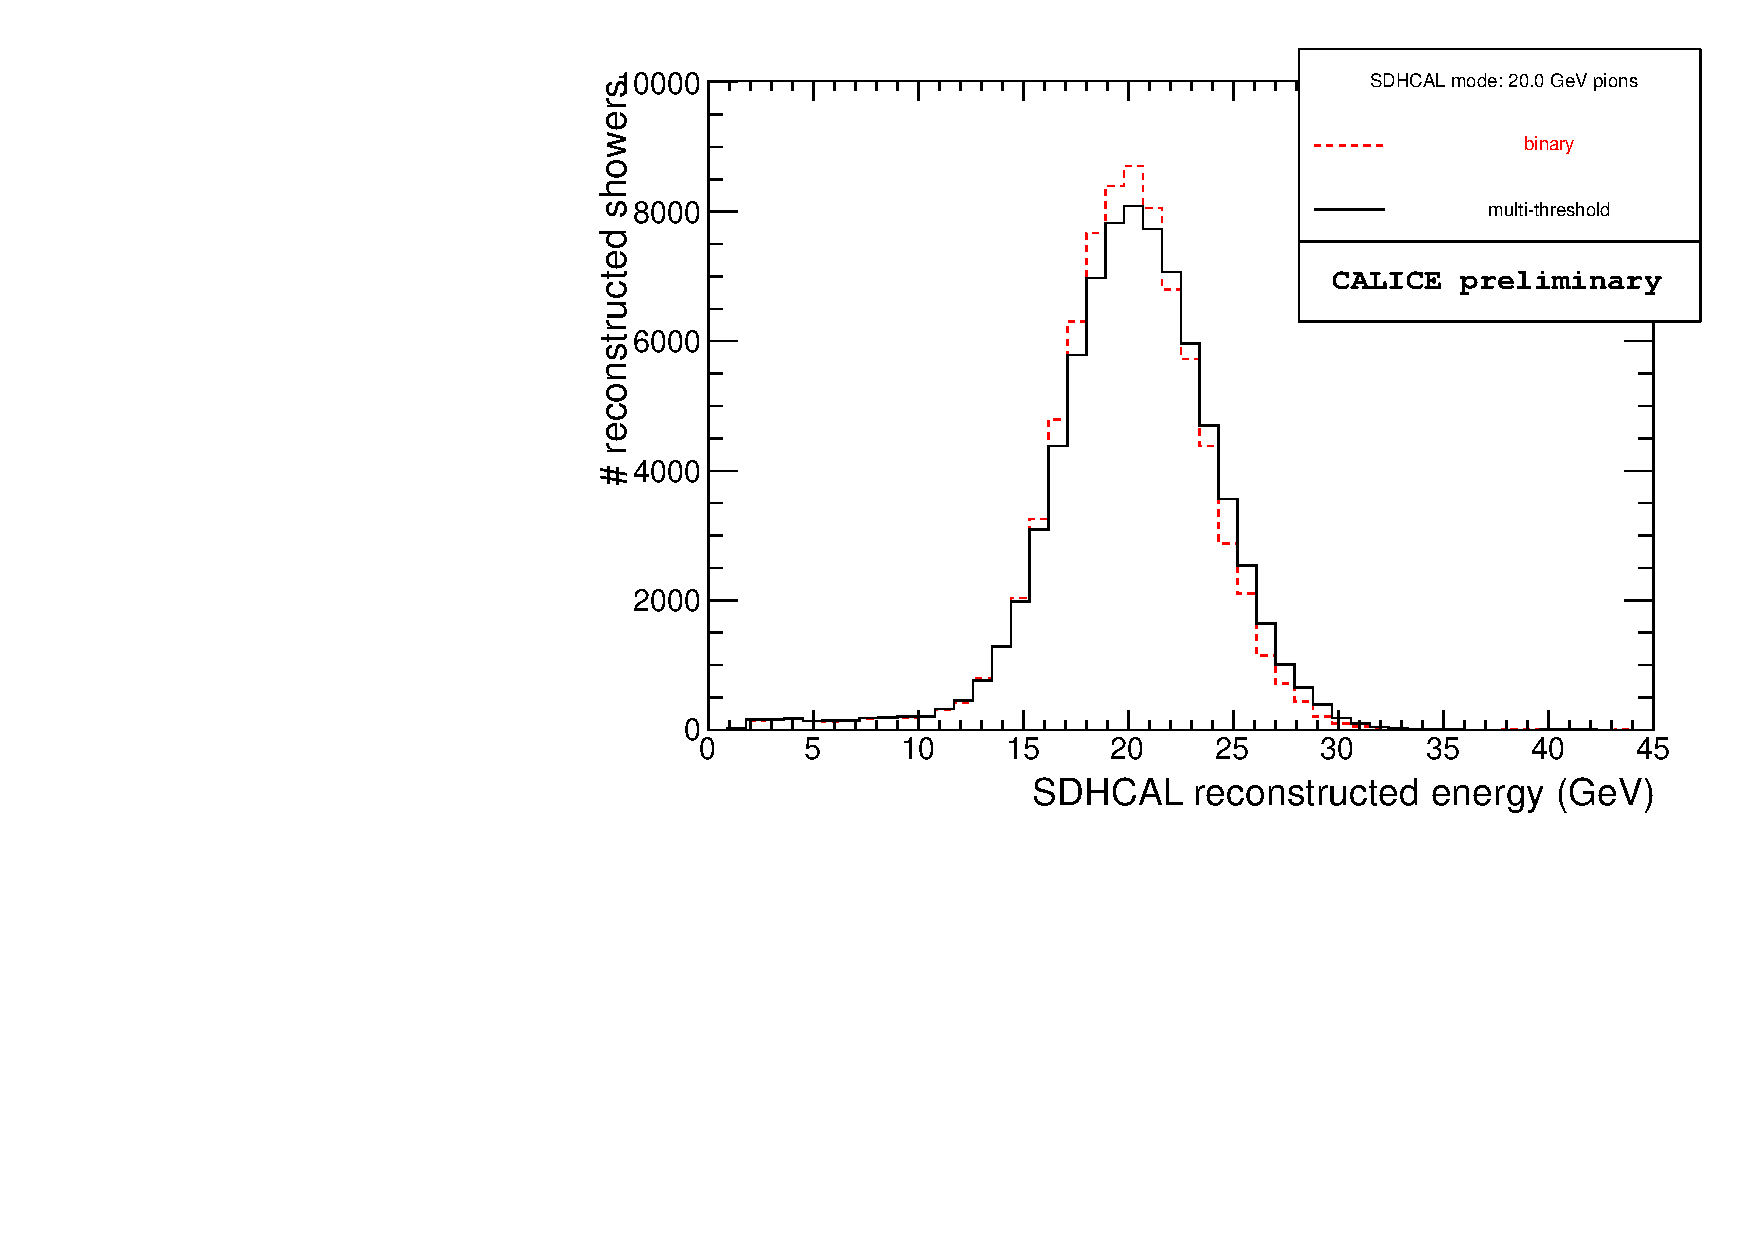
\includegraphics[width=.45\textwidth]{SDHCAL/figs/Pi20GeV_SDHCAL_2modes_overlay.pdf}
    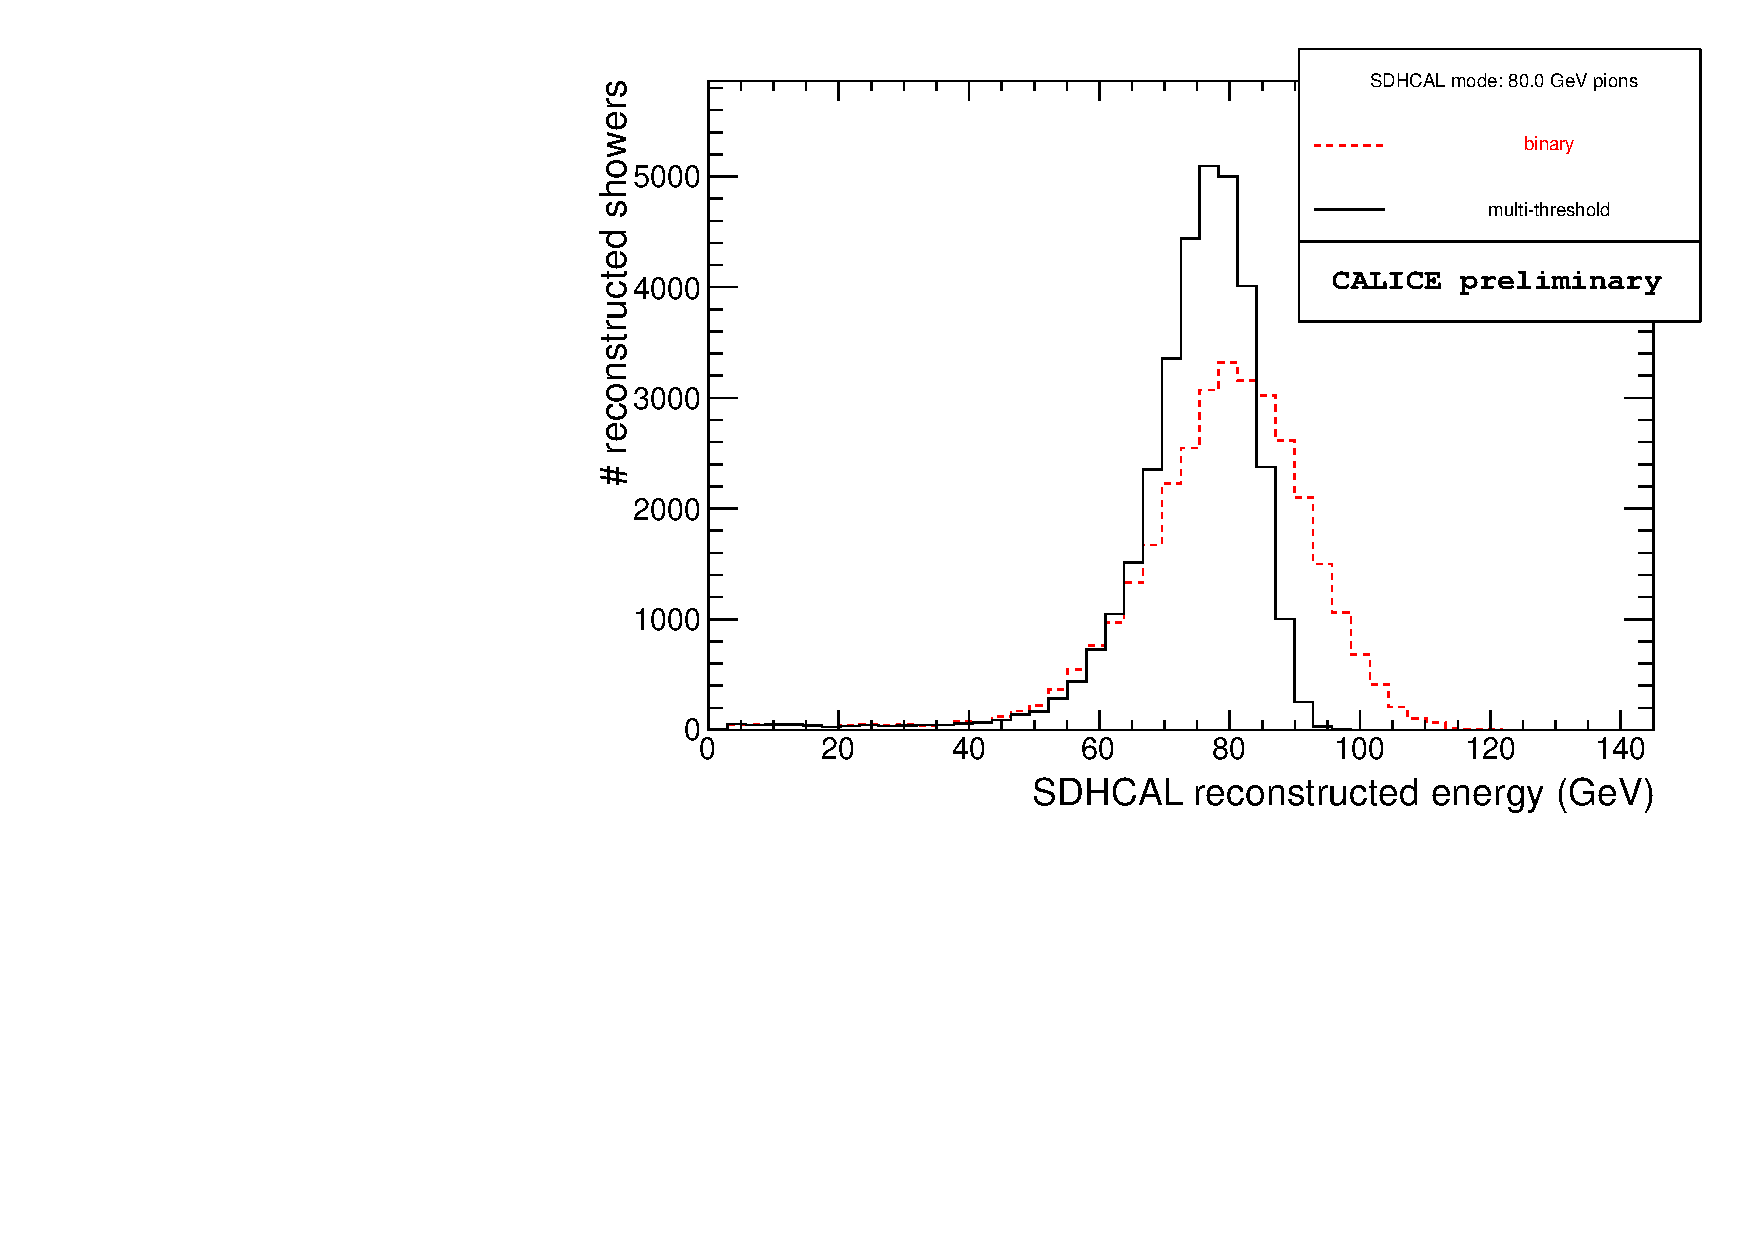
\includegraphics[width=.45\textwidth]{SDHCAL/figs/Pi80GeV_SDHCAL_2modes_overlay.pdf}
    \caption{Comparson mode binaire et multi-seuils.}
    \label{fig:multi_vs_binary}
  \end{center}
\end{figure}

\begin{figure}[!h]
  \begin{center}
    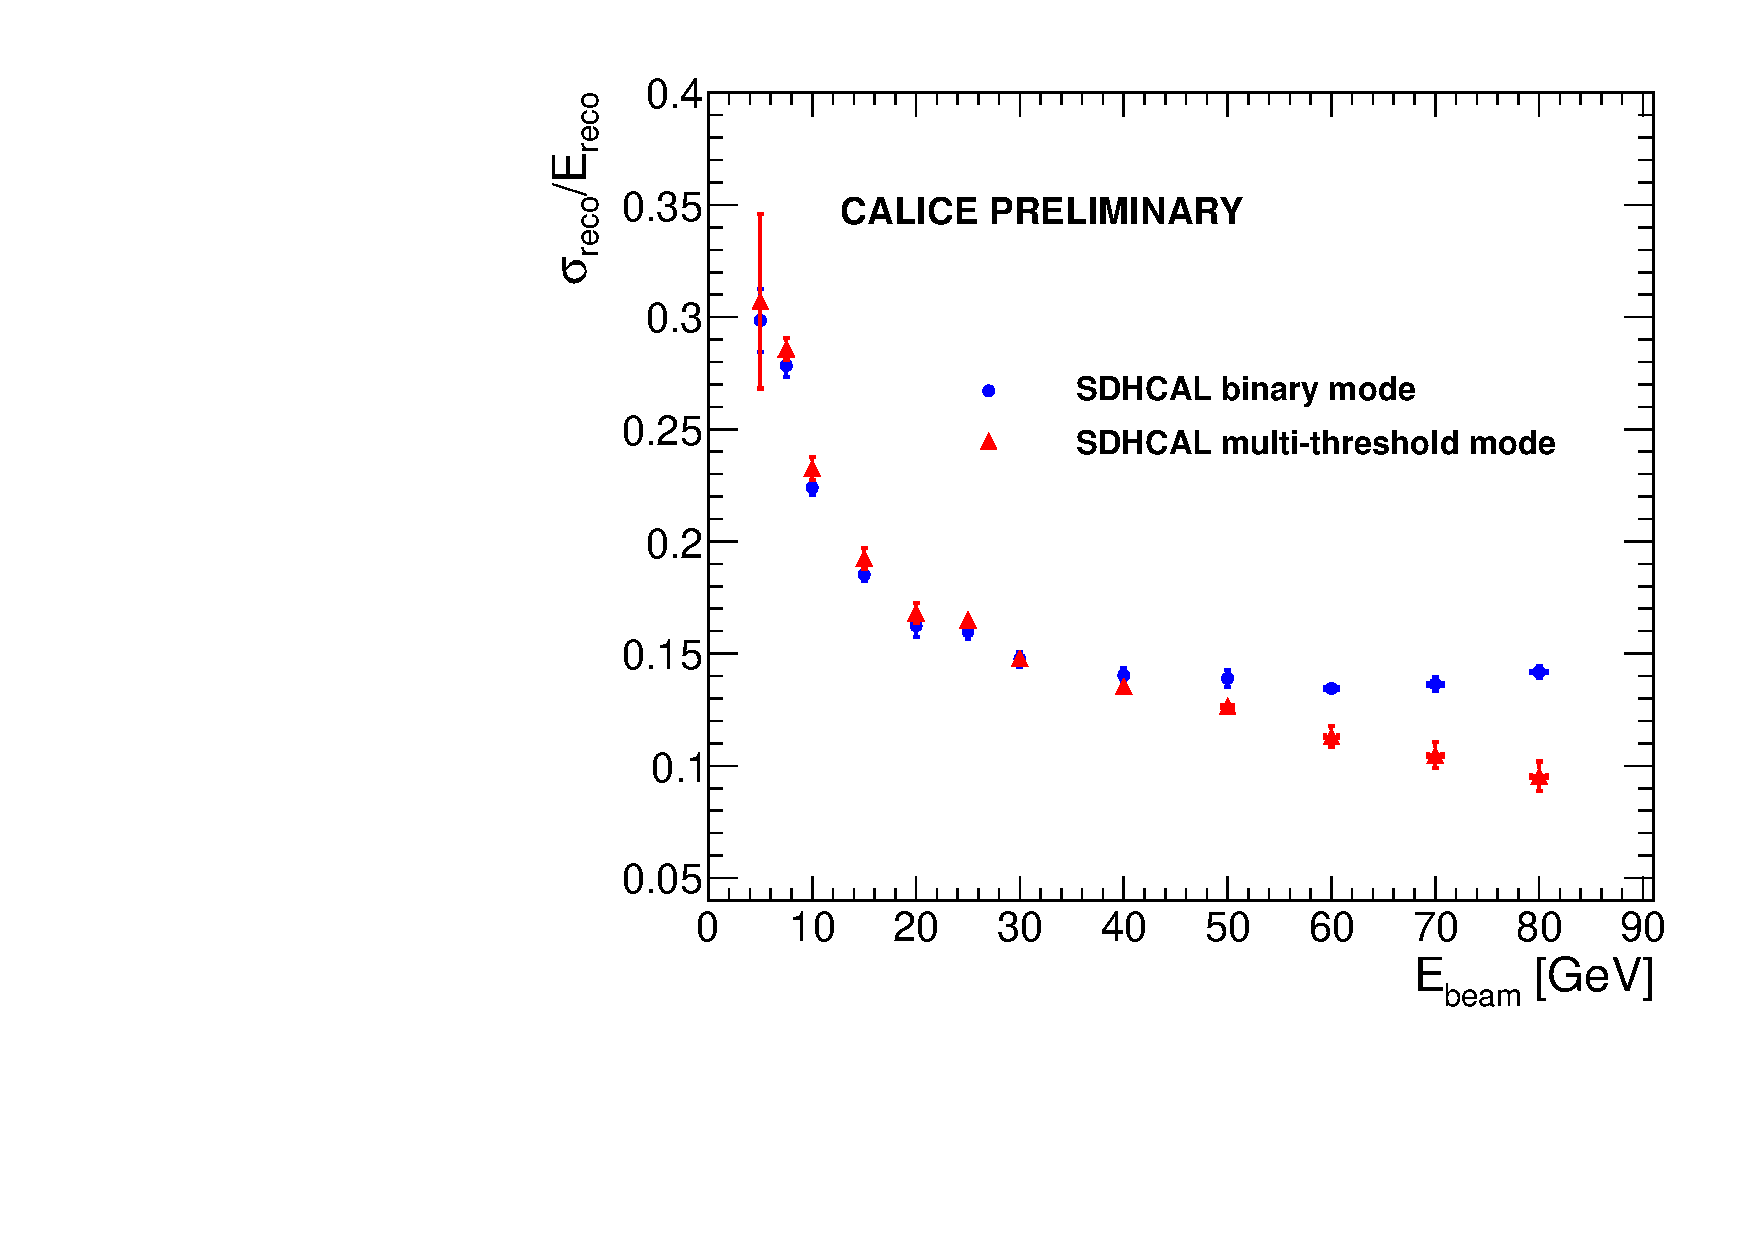
\includegraphics[width=.55\textwidth]{SDHCAL/figs/RESOLUTION.pdf}
    \caption{Résolution en energie en fonction de l'energie du faisceau pour le mode binaire et multi-seuils.}
    \label{fig:multi_vs_binary}
  \end{center}
\end{figure}
